% Generated by LitigCharts.PublicationFigures. Captions and provenance are sidecars.
\documentclass[10pt,tikz,border=5pt]{standalone}
\usepackage{lmodern}
\usetikzlibrary{patterns,patterns.meta}
\begin{document}
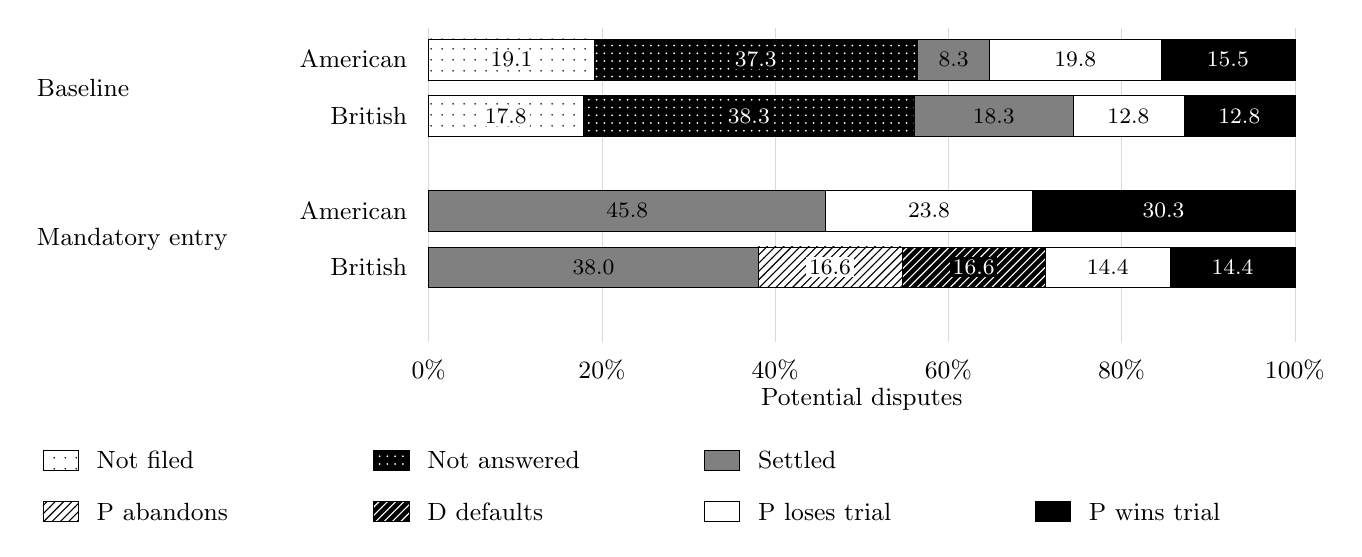
\begin{tikzpicture}[font=\small]\draw[black!15,line width=.2pt] (5.1,.65) -- (5.1,4.64);
\node[anchor=north] at (5.1,.55) {0\%};
\draw[black!15,line width=.2pt] (7.3,.65) -- (7.3,4.64);
\node[anchor=north] at (7.3,.55) {20\%};
\draw[black!15,line width=.2pt] (9.5,.65) -- (9.5,4.64);
\node[anchor=north] at (9.5,.55) {40\%};
\draw[black!15,line width=.2pt] (11.7,.65) -- (11.7,4.64);
\node[anchor=north] at (11.7,.55) {60\%};
\draw[black!15,line width=.2pt] (13.9,.65) -- (13.9,4.64);
\node[anchor=north] at (13.9,.55) {80\%};
\draw[black!15,line width=.2pt] (16.1,.65) -- (16.1,4.64);
\node[anchor=north] at (16.1,.55) {100\%};
\node[anchor=west,text width=3cm,align=left] at (0,3.88) {\mbox{Baseline}};
\node[anchor=east] at (4.95,4.24) {American};
\path[preaction={fill=white,draw=none},pattern={Dots[distance=4pt,radius=.35pt]},pattern color=black,draw=black,line width=.25pt] (5.1,3.98) rectangle (7.201583,4.5);
\node[text=black,fill=white,font=\footnotesize,inner sep=1pt] at (6.150792,4.24) {19.1};
\path[preaction={fill=black,draw=none},pattern={Dots[distance=2.8pt,radius=.35pt]},pattern color=white,draw=black,line width=.25pt] (7.201583,3.98) rectangle (11.306552,4.5);
\node[text=white,fill=black,font=\footnotesize,inner sep=1pt] at (9.254068,4.24) {37.3};
\path[fill=black!50,draw=black,line width=.25pt] (11.306552,3.98) rectangle (12.224401,4.5);
\node[text=black,fill=none,font=\footnotesize,inner sep=1pt] at (11.765476,4.24) {8.3};
\path[fill=white,draw=black,line width=.25pt] (12.224401,3.98) rectangle (14.399101,4.5);
\node[text=black,fill=none,font=\footnotesize,inner sep=1pt] at (13.311751,4.24) {19.8};
\path[fill=black,draw=black,line width=.25pt] (14.399101,3.98) rectangle (16.099998,4.5);
\node[text=white,fill=none,font=\footnotesize,inner sep=1pt] at (15.249549,4.24) {15.5};
\node[anchor=east] at (4.95,3.52) {British};
\path[preaction={fill=white,draw=none},pattern={Dots[distance=4pt,radius=.35pt]},pattern color=black,draw=black,line width=.25pt] (5.1,3.26) rectangle (7.05943,3.78);
\node[text=black,fill=white,font=\footnotesize,inner sep=1pt] at (6.079715,3.52) {17.8};
\path[preaction={fill=black,draw=none},pattern={Dots[distance=2.8pt,radius=.35pt]},pattern color=white,draw=black,line width=.25pt] (7.05943,3.26) rectangle (11.273035,3.78);
\node[text=white,fill=black,font=\footnotesize,inner sep=1pt] at (9.166233,3.52) {38.3};
\path[fill=black!50,draw=black,line width=.25pt] (11.273035,3.26) rectangle (13.281745,3.78);
\node[text=black,fill=none,font=\footnotesize,inner sep=1pt] at (12.27739,3.52) {18.3};
\path[fill=white,draw=black,line width=.25pt] (13.281745,3.26) rectangle (14.690878,3.78);
\node[text=black,fill=none,font=\footnotesize,inner sep=1pt] at (13.986312,3.52) {12.8};
\path[fill=black,draw=black,line width=.25pt] (14.690878,3.26) rectangle (16.1,3.78);
\node[text=white,fill=none,font=\footnotesize,inner sep=1pt] at (15.395439,3.52) {12.8};
\node[anchor=west,text width=3cm,align=left] at (0,1.96) {\mbox{Mandatory} \mbox{entry}};
\node[anchor=east] at (4.95,2.32) {American};
\path[fill=black!50,draw=black,line width=.25pt] (5.1,2.06) rectangle (10.142741,2.58);
\node[text=black,fill=none,font=\footnotesize,inner sep=1pt] at (7.621371,2.32) {45.8};
\path[fill=white,draw=black,line width=.25pt] (10.142741,2.06) rectangle (12.764151,2.58);
\node[text=black,fill=none,font=\footnotesize,inner sep=1pt] at (11.453446,2.32) {23.8};
\path[fill=black,draw=black,line width=.25pt] (12.764151,2.06) rectangle (16.1,2.58);
\node[text=white,fill=none,font=\footnotesize,inner sep=1pt] at (14.432076,2.32) {30.3};
\node[anchor=east] at (4.95,1.6) {British};
\path[fill=black!50,draw=black,line width=.25pt] (5.1,1.34) rectangle (9.28528,1.86);
\node[text=black,fill=none,font=\footnotesize,inner sep=1pt] at (7.19264,1.6) {38.0};
\path[preaction={fill=white,draw=none},pattern={north east lines},pattern color=black,draw=black,line width=.25pt] (9.28528,1.34) rectangle (11.109084,1.86);
\node[text=black,fill=white,font=\footnotesize,inner sep=1pt] at (10.197182,1.6) {16.6};
\path[preaction={fill=black,draw=none},pattern={north east lines},pattern color=white,draw=black,line width=.25pt] (11.109084,1.34) rectangle (12.932954,1.86);
\node[text=white,fill=black,font=\footnotesize,inner sep=1pt] at (12.021019,1.6) {16.6};
\path[fill=white,draw=black,line width=.25pt] (12.932954,1.34) rectangle (14.516481,1.86);
\node[text=black,fill=none,font=\footnotesize,inner sep=1pt] at (13.724717,1.6) {14.4};
\path[fill=black,draw=black,line width=.25pt] (14.516481,1.34) rectangle (16.099986,1.86);
\node[text=white,fill=none,font=\footnotesize,inner sep=1pt] at (15.308233,1.6) {14.4};
\node at (10.6,-.08) {Potential disputes};
\path[preaction={fill=white,draw=none},pattern={Dots[distance=4pt,radius=.35pt]},pattern color=black,draw=black,line width=.25pt] (0.2,-0.98) rectangle (0.65,-0.72);
\node[anchor=west] at (0.76,-0.85) {Not filed};
\path[preaction={fill=black,draw=none},pattern={Dots[distance=2.8pt,radius=.35pt]},pattern color=white,draw=black,line width=.25pt] (4.4,-0.98) rectangle (4.85,-0.72);
\node[anchor=west] at (4.96,-0.85) {Not answered};
\path[fill=black!50,draw=black,line width=.25pt] (8.6,-0.98) rectangle (9.05,-0.72);
\node[anchor=west] at (9.16,-0.85) {Settled};
\path[preaction={fill=white,draw=none},pattern={north east lines},pattern color=black,draw=black,line width=.25pt] (0.2,-1.63) rectangle (0.65,-1.37);
\node[anchor=west] at (0.76,-1.5) {P abandons};
\path[preaction={fill=black,draw=none},pattern={north east lines},pattern color=white,draw=black,line width=.25pt] (4.4,-1.63) rectangle (4.85,-1.37);
\node[anchor=west] at (4.96,-1.5) {D defaults};
\path[fill=white,draw=black,line width=.25pt] (8.6,-1.63) rectangle (9.05,-1.37);
\node[anchor=west] at (9.16,-1.5) {P loses trial};
\path[fill=black,draw=black,line width=.25pt] (12.8,-1.63) rectangle (13.25,-1.37);
\node[anchor=west] at (13.36,-1.5) {P wins trial};
\end{tikzpicture}
\end{document}
